\documentclass[11pt,letterpaper]{article}
\usepackage[utf8]{inputenc}
\usepackage[top=1in,bottom=1in,left=1in,right=1in]{geometry}
\usepackage{amsmath}
\usepackage{amsfonts}
\usepackage{amssymb}
\usepackage{amsthm}
\usepackage{bm}
\usepackage{braket}
\usepackage{cancel}
\usepackage{enumitem}
\usepackage{float}
\usepackage{graphicx}
\usepackage{hyperref}
\usepackage{mathabx}
\usepackage{parskip}
\usepackage{tensor}
\usepackage{titlesec}
\usepackage{titling}
\usepackage{listings}


% \setenumerate{leftmargin=*,label=\bf(\alph*)}


\titlelabel{(\thetitle)\quad}
\titleformat*{\section}{\large\bfseries}
\titleformat*{\subsection}{\normalsize\bfseries}
\setlength{\droptitle}{-5em}



\let\Re\relax
\DeclareMathOperator{\Re}{Re}
\let\Im\relax
\DeclareMathOperator{\Im}{Im}

\DeclareMathOperator{\diag}{diag}


\newcommand{\bhat}[1]{\hat{\bm{#1}}}


\renewcommand{\thesubsection}{\normalsize \alph{subsection}}
\renewcommand{\d}{\mathrm{d}}
\renewcommand{\vec}[1]{\bm{#1}}
\newcommand{\del}{\vec{\nabla}}
\newcommand{\e}{\epsilon}
\newcommand{\tpd}[3]{\left( \frac{\partial #1}{\partial #2} \right)_{#3}}
\newcommand{\pd}[2]{\frac{\partial #1}{\partial #2}}
\newcommand{\spd}[2]{\frac{\partial^2 #1}{\partial {#2}^2}}
\def\dbar{{\mathchar'26\mkern-12mu d}}

\allowdisplaybreaks


\author{Sam Kowash}
\numberwithin{equation}{section}
\numberwithin{figure}{section}
\title{CSE 546 HW \#0}

\begin{document}
\maketitle

\section{Analysis}
\begin{enumerate}
	\item A set $A \subseteq \mathbb{R}^n$ is convex if $\lambda x + (1-\lambda)y \in A$ for all $x,y\in A$. A norm $\|\cdot\|$ on $\mathbb{R}^n$ is non-negative, absolutely scalable, and satisfies the triangle inequality.
		\begin{enumerate}
		\item 
		Let $A = \{x \in \mathbb{R}^n : \|x\| \leq 1\}$ for some norm $\|\cdot\|$, take $x,y \in A$, and take $\lambda \in [0,1]$. By the triangle inequality,
		%
		\begin{align*}
			\|\lambda x + (1-\lambda)y\| &\leq \|\lambda x\| + \|(1-\lambda)y\|.
		\end{align*}
		%
		Scalability then tells us
		%
		\begin{align*}
			 \|\lambda x\| + \|(1-\lambda)y\| &= |\lambda| \|x\| + |1-\lambda|\|y\|,
		\end{align*}
		%
		and since $0 \leq \|x\|,\|y\| \leq 1$,
		%
		\begin{align*}
			|\lambda| \|x\| + |1-\lambda|\|y\| &\leq |\lambda| + |1-\lambda|.
		\end{align*}
		%
		Lastly, with $\lambda \in [0,1]$, $|\lambda|=\lambda$ and $|1-\lambda|=1-\lambda$, so by applying transitivity through the chain of (in)equalities, we find
		%
		\begin{align*}
			\|\lambda x + (1-\lambda)y\| &\leq 1,
		\end{align*}
		%
		so $\lambda x + (1-\lambda)y \in A$ and $A$ is convex, regardless of the norm used.




		\item
		Consider the function $f(x) = \left(\sum_{i=1}^n |x_i|^\frac{1}{2}\right)^2$ for $x\in \mathbb{R}^n$. It is clearly non-negative for all inputs since it is a square of a sum of real numbers. Further, it is absolutely scalable, since a factor $\lambda$ will come out of the sum as $\sqrt{|\lambda|}$, then be squared to give an overall scaling $|\lambda|$. However, consider $x = (1,0,0,\ldots,0)$ and $y = (0,1,0,\ldots,0)$. We have $f(x)= f(y) = 1$, but $f(x+y) = (\sqrt{1}+\sqrt{1})^2 = 4$, so $f(x+y) > f(x)+f(y)$ meaning that this function does not satisfy the triangle inequality and \emph{cannot be a norm}. (We can also see this by plotting a level set of this function and noting that the region bounded by it is non-convex, in contradiction to the previous result.)
	\end{enumerate}



	\item For $x \in \mathbb{R}^n$, define the norms
	%
	\begin{align*}
		\|x\|_1 &= \sum_{i=1}^n |x_i|,&
		\|x\|_2 &= \sqrt{\sum_{i=1}^n |x_i|^2},&
		\|x\|_\infty &= \max_{i=1,\ldots,n} |x_i|.
	\end{align*}
	%
	Each norm must obey the triangle inequality, so in particular (if we apply the inequality repeatedly),
	%
	\begin{align*}
		\|x\| = \left\|\sum_{i=1}^n x_i e_i\right\| \leq \sum_{i=1}^n \|x_i e_i\| = \sum_{i=1}^n |x_i| = \|x\|_1,
	\end{align*}
	%
	where $e_i$ are unit basis vectors with respect to the given norm and the second equality comes by absolute scalability. Thus, we see that no norm exceeds the Manhattan norm. Further,
	%
	\begin{align*}
		\|x\|_2 = \sqrt{\sum_{i=1}^n |x_i|^2} \geq \sqrt{(\max_{i=1,\ldots,n} |x_i|)^2} = \max_{i=1,\ldots,n} |x_i| = \|x\|_\infty,
	\end{align*}
	%
	so the infinity norm cannot exceed the Euclidean norm. This gives the ranking \mbox{$\|x\|_\infty \leq \|x\|_2 \leq \|x\|_1$}, as desired.





	\item For $A,B \in \mathbb{R}^{n\times n}$, $c \in \mathbb{R}$, and $f(x,y) = x^T A x + y^T B x + c$ acting on $x,y \in \mathbb{R}^n$, we define the derivative
	%
	\begin{align*}
		\nabla_z f(x,y) = \begin{bmatrix}\pd{f(x,y)}{z_1} & \pd{f(x,y)}{z_2} & \cdots & \pd{f(x,y)}{z_n}\\\end{bmatrix}^T.
	\end{align*}
	%
	It will be cleaner to compute these derivatives with matrix operations expressed component-wise, so for the rest of this problem we adopt Einstein summation notation wherein repeated indices are summed over. We will also use $\partial_{z_i}$ to denote $\pd{}{z_i}$. Then,
	%
	\begin{align*}
		(\nabla_x f(x,y))_i &= \partial_{x_i} \left(A_{jk} x_j x_k + B_{jk} y_j x_k + c\right)\\
		&= \delta_{ij} A_jk x_k + \delta_{ik} A_jk x_j + \delta_{ik} B_{jk} y_j\\
		&= A_{ik} x_k + x_j A_{ji} + y_j B_{ji},
	\end{align*}
	%
	so, returning to matrix notation,
	%
	\begin{align}
		\nabla_x f(x,y) &= (A+A^T)x +B^Ty.
	\end{align}
	%
	Similarly,
	%
	\begin{align*}
		(\nabla_y f(x,y))_i &= \partial_{y_i} \left(A_{jk} x_j x_k + B_{jk} y_j x_k + c\right)\\
		&= \delta_{ij} B_{jk} x_k\\
		&= B_{ik} x_k,
	\end{align*}
	%
	so
	%
	\begin{align*}
		\nabla_y f(x,y) &= Bx.
	\end{align*}








	\item Let $A,B \in \mathbb{R}^{n\times n}$ be symmetric matrices sharing eigenvectors $u_1,\ldots,u_n$ with corresponding eigenvalues $\alpha_1,\ldots,\alpha_n$ for $A$ and $\beta_1,\ldots,\beta_n$ for $B$.

	\begin{enumerate}
		\item The matrix $C = A+B$ shares the eigenvectors $u_1,\ldots,u_n$, with eigenvalues \mbox{$\alpha_1+\beta_1,\ldots,\alpha_n+\beta_n$}.
		\item The matrix $D = A-B$ shares the eigenvectors $u_1,\ldots,u_n$, with eigenvalues \mbox{$\alpha_1-\beta_1,\ldots,\alpha_n-\beta_n$}.
		\item The matrix $E=AB$ shares the eigenvectors $u_1,\ldots,u_n$, with eigenvalues \mbox{$\alpha_1\beta_1,\ldots,\alpha_n\beta_n$}.
		\item Assuming that $A$ is nonsingular, the matrix $F = A^{-1}B$ shares the eigenvectors $u_1,\ldots,u_n$, with eigenvalues \mbox{$\frac{\beta_1}{\alpha_1},\ldots,\frac{\beta_n}{\alpha_n}$}.
	\end{enumerate}







	\item A symmetric matrix $A \in \mathbb{R}^{n\times n}$ is positive-semidefinite (PSD) if $x^T A x \geq 0$ for all $x \in \mathbb{R}^n$.
	\begin{enumerate}
		\item Let $y\in \mathbb{R}^n$. For any $x\in \mathbb{R}^n$, note that $x^T y = y^T x$, so
		%
		\begin{align*}
			x^T y y^T x = (y^T x)^2 \geq 0,
		\end{align*}
		%
		so $y y^T$ is PSD.

		\item Let $X$ be a random vector in $\mathbb{R}^n$ with covariance matrix $\Sigma = \mathbb{E}\left[(X-\mathbb{E}[X])(X-\mathbb{E}[X])^T\right]$. By the previous result, $(X-\mathbb{E}[X])(X-\mathbb{E}[X])^T$ is PSD since it's the outer product of a vector with itself. Sums of PSD matrices must be PSD, so any linear combination of PSD matrices with non-negative weights is in turn PSD. The expected value is such a combination, with weights given by the PDF of $X$, so $\Sigma$ is PSD.

		\item Take $A$ to be a symmetric matrix so that (by the real spectral theorem) there exist an orthogonal matrix $U$ and list of eigenvalues $\alpha$ satisfying $A = U \diag(\alpha) U^T$. The columns of $U$ form basis for $\mathbb{R}^n$, so we can decompose any vector $x\in\mathbb{R}^n$ as $x = \sum_i c_i u_i$, where $c_i$ are scalars and $u_i$ are the columns of $U$. Because that basis is in fact orthonormal, we know that $Uu_i = e_i$, so
		%
		\begin{align*}
			x^T A x &= \left(\sum_{i} c_i u_i^T\right) U \diag(\alpha) U^T \left(\sum_{j} c_j u_j \right)\\
			x^T A x &= \left(\sum_i c_i e_i^T\right) \diag(\alpha) \left(\sum_j c_j e_j\right)\\
			x^T A x &= \sum_i c_i^2 \alpha_i,
		\end{align*}
		%
		where orthonormality collapses one of the sums. The resulting sum can only be non-negative for all choices of components $c_i$ if the eigenvalues $\alpha_i$ are each non-negative, which is to say that $\min_i \alpha_i \geq 0$.
	\end{enumerate}





	\item Consider real independent variables $X$ and $Y$ with PDFs $f$ and $g$, respectively. Let $h$ be the PDF of $Z = X+Y$.
	\begin{enumerate}
		\item The PDF for the sum of $X$ and $Y$ will be the convolution of their respective PDFs:
		%
		\begin{align*}
			h(x) &= \int_{-\infty}^\infty f(y) g(x-y) \d y.
		\end{align*}
		%
		We can understand this as accounting for the probabilities of all of the different ways that outcomes of $X$ and $Y$ can add to a particular outcome $x$ of $Z$.

		\item In particular we take $X$ and $Y$ both uniformly distributed on $[0,1]$. It is easy to think about the convolution geometrically as sliding one unit square past the other and measuring the area of overlap. This falls to zero outside of $(0,2)$ and rises to a maximum of 1 at $x=1$, with linear change in between, so we can write
		%
		\begin{align*}
			h(x) &= \left\{\begin{array}{ll}
			x &: 0\leq x \leq 1\\
			2-x &: 1 < x \leq 2\\
			0 &: \text{else}
			\end{array}\right..
		\end{align*}


		\item We now wish to find $\mathbb{P}(X\leq1/2 \mid X+Y \geq 5/4)$ for these distributions. This, too, we can think of geometrically: if we put values of $X$ on the $x$-axis and those of $Y$ on the $y$-axis, the joint distribution has support on the unit square in the first quadrant. The event $X+Y \geq 5/4$ has probability equal to the area of the upper triangle bounded by $y=5/4-x$, and $(X \leq 1/2) \cap (X+Y \geq 5/4)$ is the portion of that triangle in the left half of the unit square. The diagonal boundary line for the triangle meets the edges of the square at $(1,1/4)$ and $(1/4,1)$, so the triangle has base and height $3/4$ and so  area $9/32$. The smaller triangle has base and height $1/4$ and area $1/32$, so the conditional probability is $1/9$. See Fig.~'\ref{fig:condprob} for clarification.

		\begin{figure}[H]
			\centering
			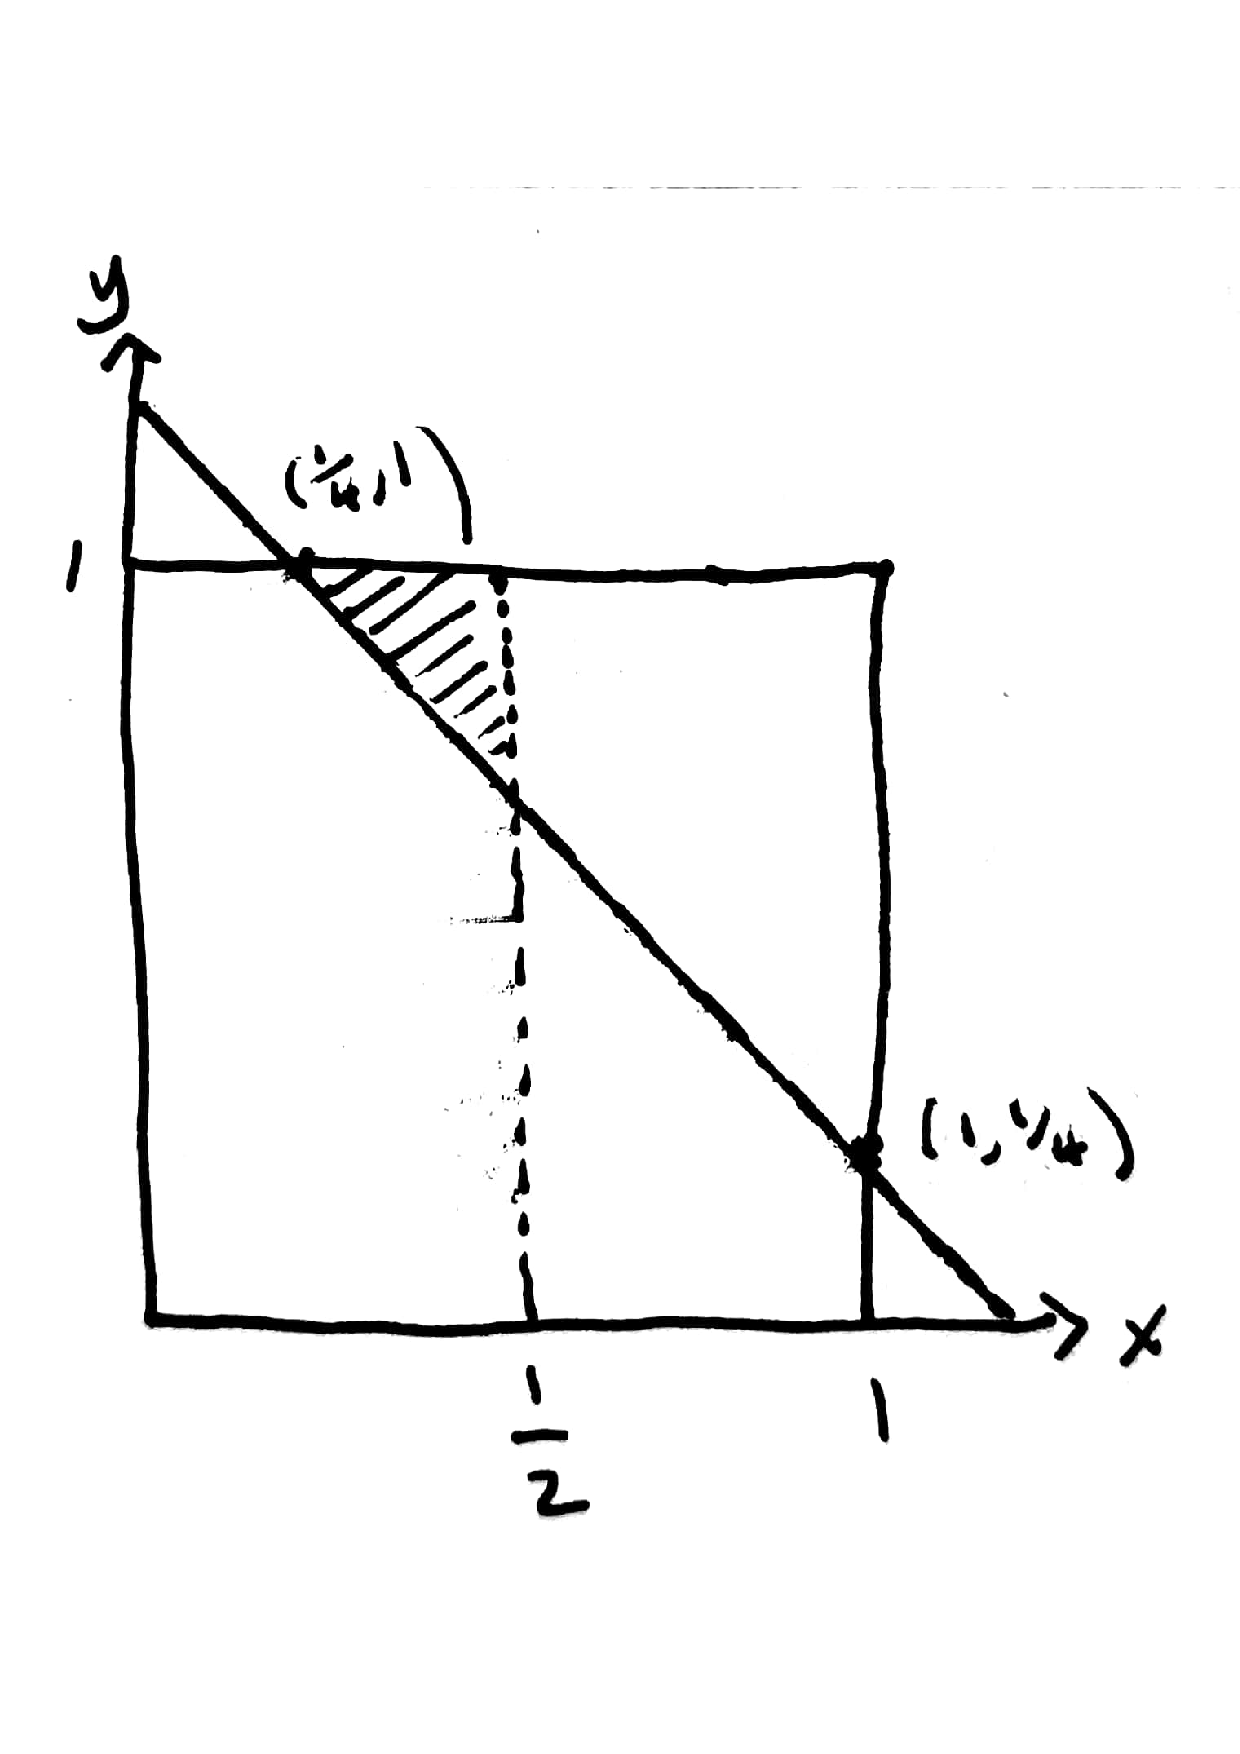
\includegraphics[width=.3\textwidth]{figures/condprob.pdf}
			\caption{Geometry of conditional probability calculation}
			\label{fig:condprob}
		\end{figure}
	\end{enumerate}




	\item Given a random variable $X \sim \mathcal{N}(\mu,\sigma^2)$, we wish to define $Y = aX + b$ such that $Y \sim \mathcal{N}(0,1)$. We can do this just by inspecting the differential probability 
	%
	\begin{align*}
		\d \mathbb{P}(x) &= \frac{1}{\sqrt{2\pi \sigma^2}} \exp\left[-\frac{(x-\mu)^2}{2\sigma^2}\right] \d x.
	\end{align*}
	%
	If we define $x = \frac{y-b}{a}$, we see
	%
	\begin{align*}
		\d \mathbb{P}(y) &= \frac{1}{\sqrt{2\pi \sigma^2}} \exp\left[-\frac{\left(\frac{y-b}{a}-\mu\right)^2}{2\sigma^2}\right] \frac{\d y}{a},
	\end{align*}
	%
	which we can rearrange into
	%
	\begin{align*}
		\d \mathbb{P}(y) &= \frac{1}{\sqrt{2 \pi (a \sigma)^2}} \exp\left[-\frac{\left(y-(b+a\mu)\right)^2}{2(a \sigma)^2}\right] \d y.
	\end{align*}
	%
	It is then clear that $a = 1/\sigma$ and $b = -\frac{\mu}{\sigma}$ gives a Gaussian distribution with zero mean and unit variance, as desired.



	\item Let $X_1,\ldots,X_n$ be i.i.d. random variables with CDF $F(x)$. We define ${\hat{F}_n(x) = \frac{1}{n} \sum_{i=1}^n \bm{1}\{X_i \leq x\}}$, where $\bm{1}(A)$ is the indicator function for a Boolean event $A$, which is $1$ when $A$ is true and $0$ otherwise.
	\begin{enumerate}
		\item We know that for any random variable $X$, $\mathbb{E}[\bm{1}\{X\leq x\}]$ is equal to the CDF of $X$. Since all of our $n$ variables have the same CDF,
		%
		\begin{align*}
			\mathbb{E}[\hat{F}_n(x)] &= \frac{1}{n} \sum_{i=1}^n F(x) = \frac{n F(x)}{n} = F(x).
		\end{align*}

		\item We now wish to find $\mathbb{E}[(\hat{F}_n(x) - F(x))^2]$, which by the previous result we recognize is equal to $\mathbb{E}[\hat{F}_n(x)^2] - F(x)^2$, so we should focus on computing $\mathbb{E}[\hat{F}_n^2]$.
		%
		\begin{align*}
			\left(\hat{F}_n(x)\right)^2 &= \frac{1}{n^2} \sum_{i,j=1}^n \bm{1}\{X_i\leq x\}\bm{1}\{X_j\leq x\}
		\end{align*}
		%
		This double sum has two types of terms. There are $n$ diagonal terms where $i=j$ and we get a square of an indicator function, which is just the same indicator function back again and has expectation $F(x)$. There are also ${n^2-n}$ off-diagonal terms where $i\neq j$ and we should think of the product as the indicator function for the event $(X_i \leq x) \cap (X_j \leq x)$ and its expected value as the joint CDF for $X_i$ and $X_j$. Because all of our variables are independent, that joint CDF is just the product of CDFs for the variables, which are here the same, so these off-diagonal terms give $\left(F(x)\right)^2$. Thus,
		%
		\begin{align*}
			\mathbb{E}[(\hat{F}_n(x) - F(x))^2] &= \frac{1}{n^2}\left[ nF(x) + (n^2-n)\left(F(x)\right)^2\right] - \left(F(x)\right)^2\\
			\mathbb{E}[(\hat{F}_n(x) - F(x))^2] &= \frac{F(x)\left(1-F(x)\right)}{n}.
		\end{align*}



		\item Looking at the numerator of the previous result as a quadratic function of $F(x)$, we see that it is maximal when $F(x) = 1/2$, which gives the numerator a maximum value of $1/4$. This means that
		%
		\begin{align*}
			\sup_{x\in\mathbb{R}} \mathbb{E}\left[\left(\hat{F}_n(x)-F(x)\right)^2\right] & \leq \frac{1}{4n}.
		\end{align*}
	\end{enumerate}
\end{enumerate}












\section{Programming}

\begin{enumerate}
	\setcounter{enumi}{8}
	\item We investigate the central limit theorem numerically, using the family of random variables $Y^{(k)} = \frac{1}{\sqrt{k}} \sum_{i=1}^k B_i$, where each $B_i$ takes values $-1$ and $1$ with equal probability. The last result above tells us that
		\begin{align*}
			\sup_x \sqrt{\mathbb{E}[(\hat{F}_n(x)-F(x))^2]} &\leq \frac{1}{2\sqrt{n}},
		\end{align*}
		%
	so for $n=40000$ we can guarantee that the standard deviation of the empirical CDF $\hat{F}_n(x)$ is no greater than $0.0025$.

	\begin{figure}[H]
		\centering
		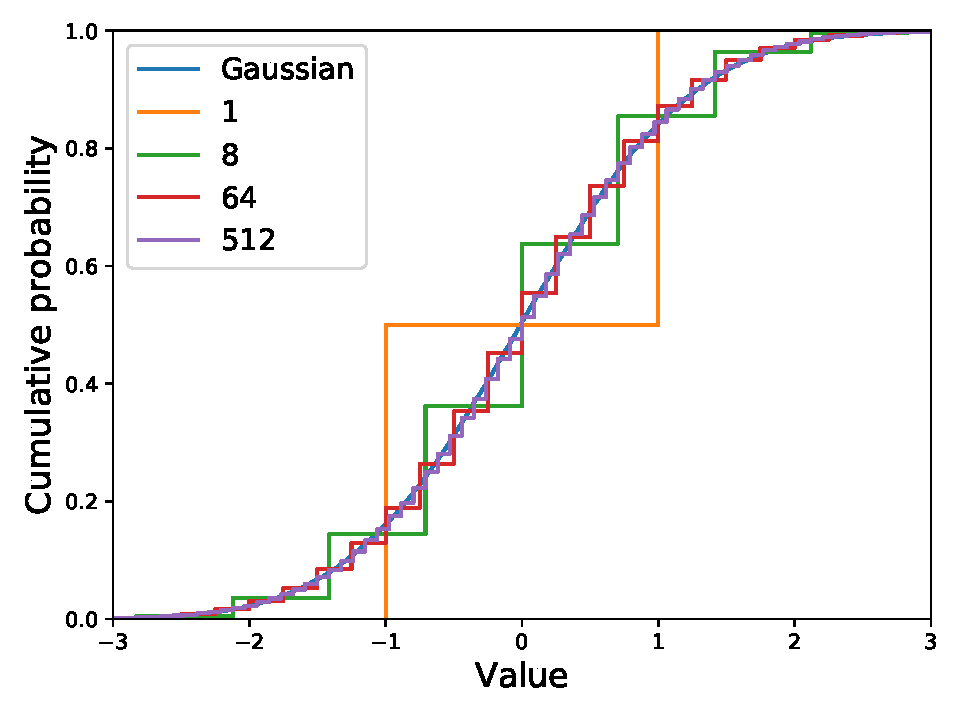
\includegraphics[width=.7\textwidth]{figures/cdfs.pdf}
		\caption{Empirical CDFs of Gaussian and of $Y^{(k)}$ for various $k$}
		\label{fig:cdfs}		
	\end{figure}

	Figure~\ref{fig:cdfs} plots the estimator $\hat{F}_n(x)$ for a Gaussian random variable and for our family $Y^{(k)}$ at various values of $k$. We can see that as $k$ increases, $\hat{F}_n^{(k)}$ tends toward $\hat{F}_n$, justifying the claim of the central limit theorem that $Y^{(k)}$ tends toward a normal random variable as $k \to \infty$. Code follows on next page.
\end{enumerate}

\clearpage

\lstinputlisting[language=Python]{code/hw0.py}

\end{document}